\subsection{Case study}\label{subsec:case-study}
This section describes the practical experiment used to evaluate representations.

\subsubsection{Scenario and context}
The goal of this experiment was to evaluate the expressiveness of representations in a practical context.
This was achieved by recreating a few screens of a fictional application.
The application designed for this experiment was modeled after Trello\furl{trello.com} \textendash\ a well-known Web application for creating Kanban-style lists.
The choice was motivated by the application's popularity and relative complexity.

Capabilities of the original are very broad and include detailed management of workspaces, users, boards, as well as editing and managing content-rich cards.
It would not be reasonable to implement all these functionalities \textendash\ \todo{write better}to keep the experiment manageable, it was necessary to limit its scope.
The selected area to implement concerned simple management of cards and spans two views and a single dialog window:
\begin{itemize}
    \item the first view allows for viewing all boards the user has access to and navigating to a board
    \item the second view allows for viewing a particular board and its data \textendash\ name, columns and cards
    \item the dialog window allows for adding or editing a single card
\end{itemize}
This setup covers all four CRUD operations, making the experiment representative of real-life applications.
Management of boards and columns within a board was omitted to keep the example as small as possible.

Additionally, the representations should be able to represent two major components:
\begin{itemize}
    \item a card \textendash\ contains information about a title of a task, its description, assigned person and due date; it is also assigned to a column
    \item a column \textendash\ a board consists of multiple columns, each possibly containing multiple cards; additionally, to give it meaning, it also has a title
\end{itemize}

To further simplify the experiment, the interface was only implemented in a mobile version \textendash\ it is considered a good practice to design applications and website using the \enquote{mobile first} principle\furl{https://developer.mozilla.org/en-US/docs/Web/Progressive_web_apps/Responsive/Mobile_first}.% \textendash\ focusing on designing for narrow devices in the first place and extending the design from there.

The subsequent paragraphs provide a detailed description of functionalities that the representations were expected to implement.

\paragraph{The boards view}
The boards view consists of\textellipsis

\paragraph{The board view}
The board view, presented in figure~\ref{fig:3-4-board-view} consists of\textellipsis

\begin{figure}
    \centering
    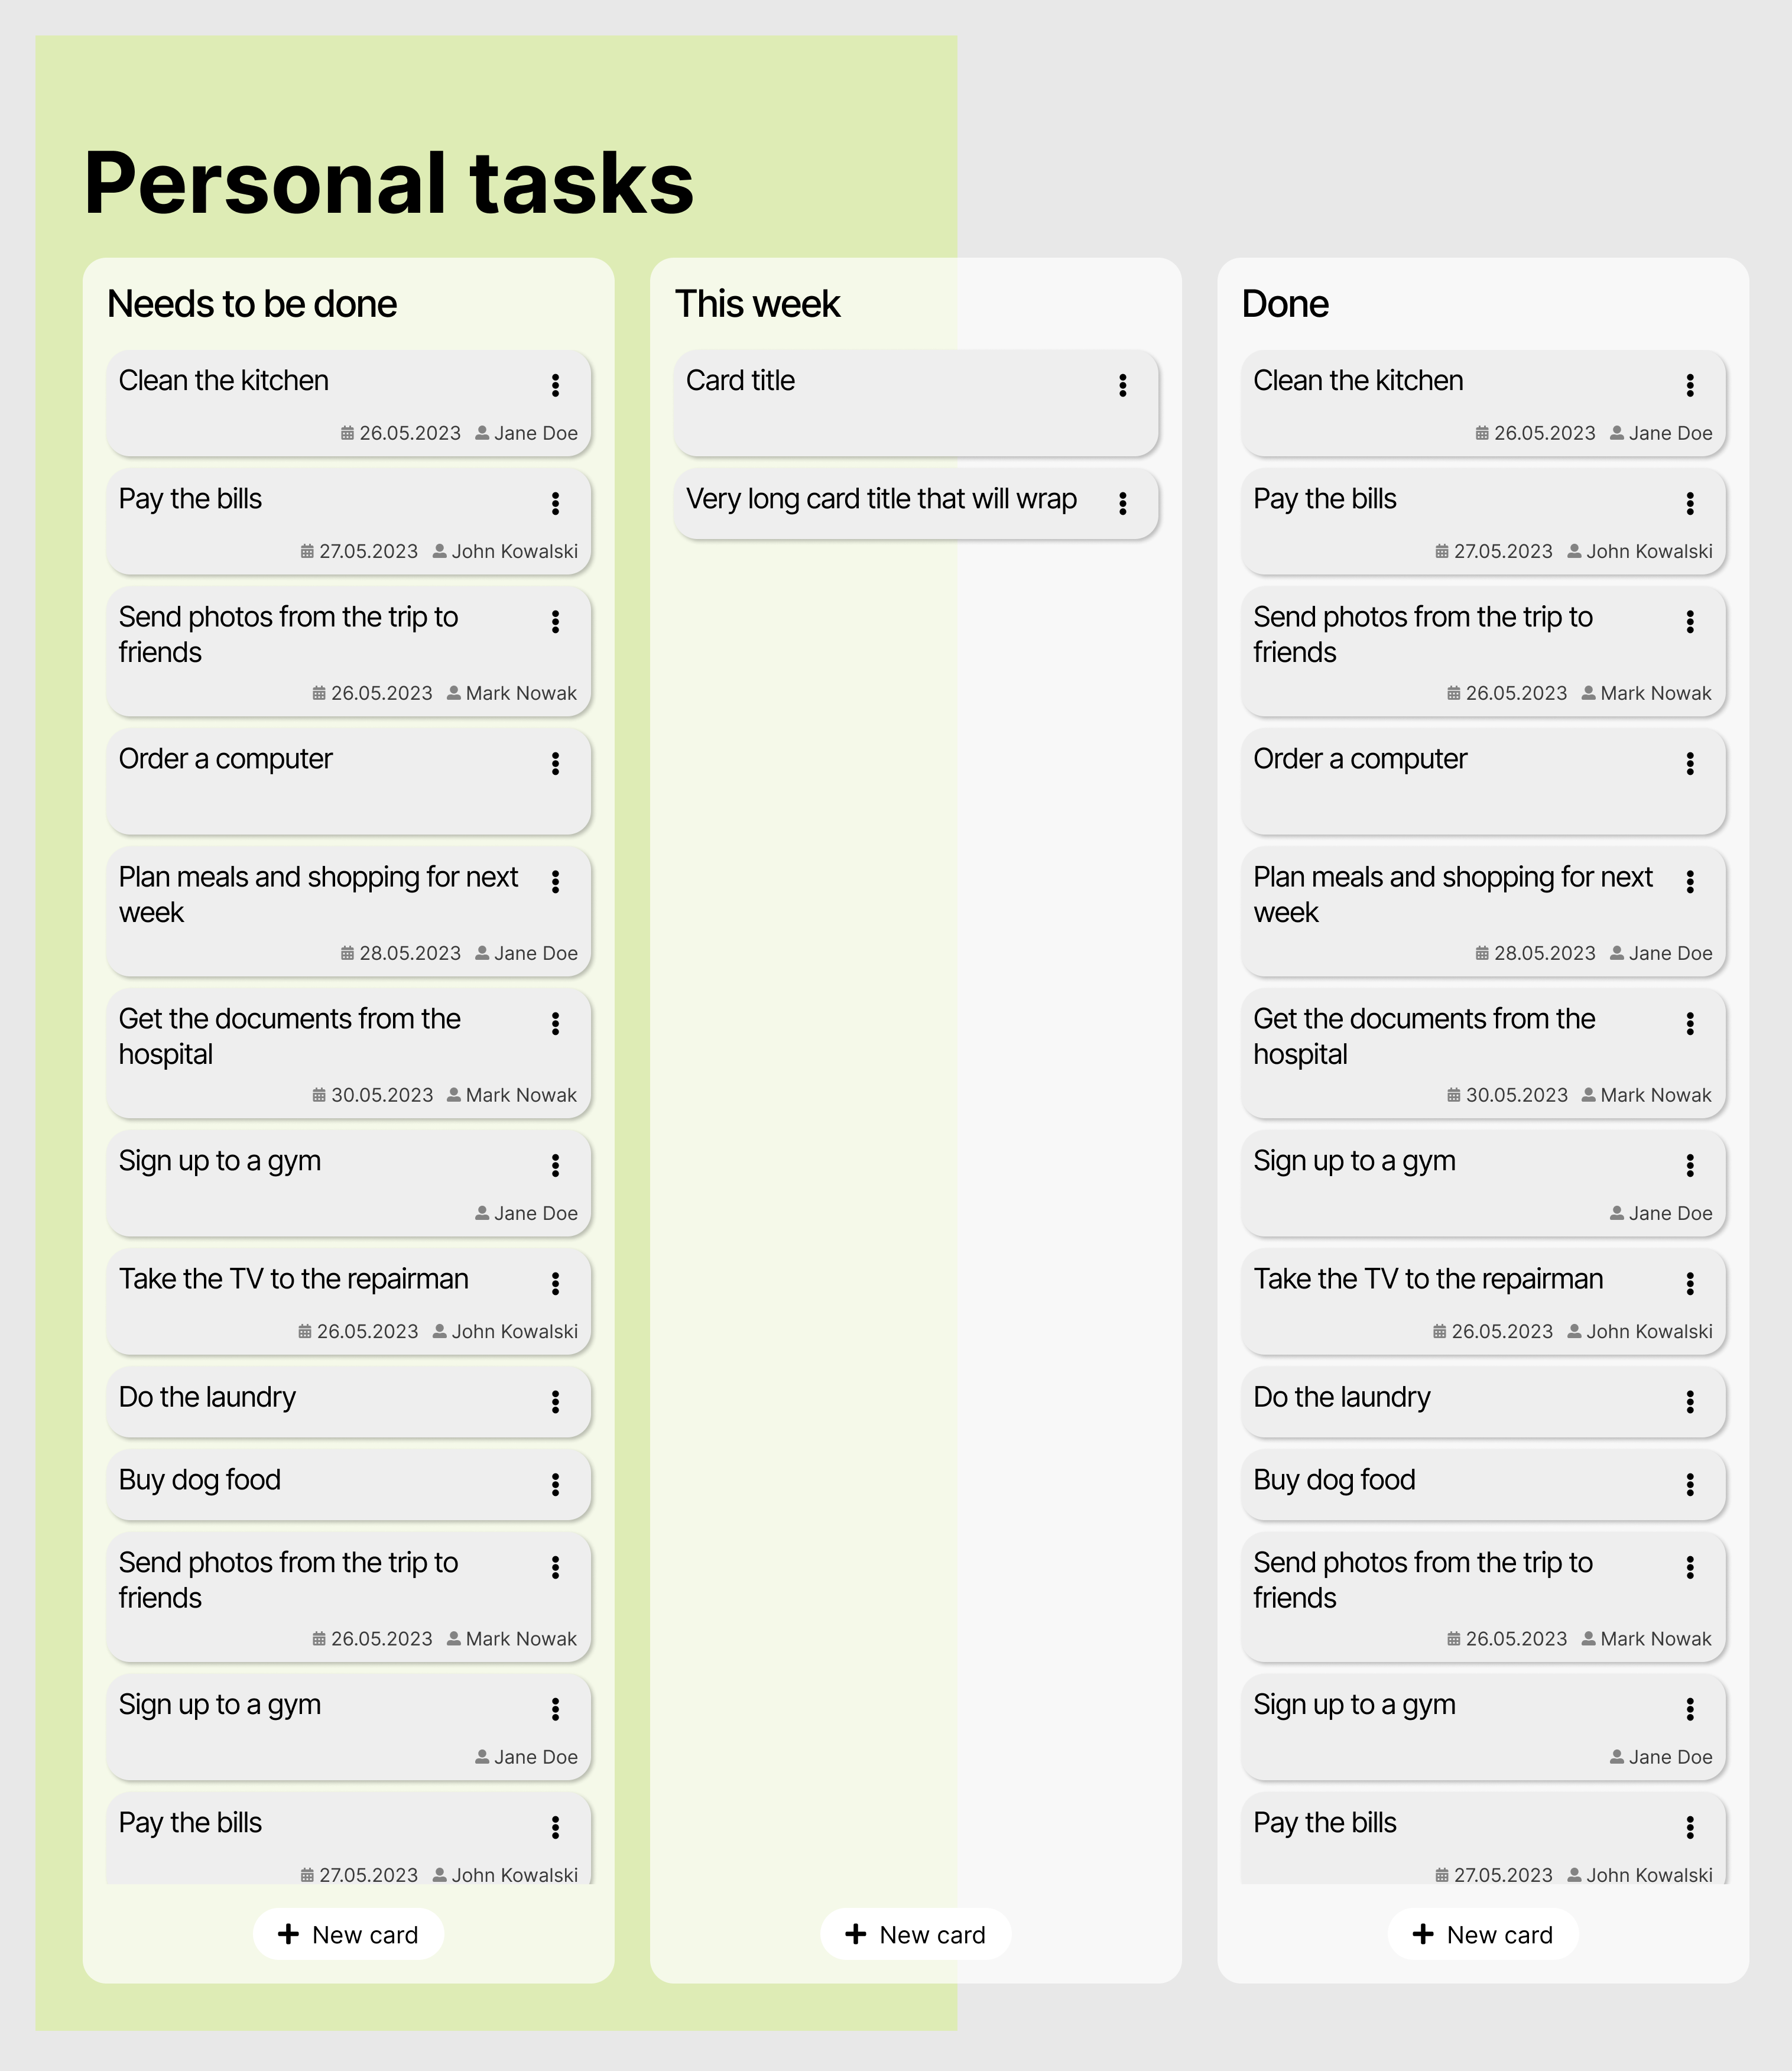
\includegraphics[height=0.5\textheight]{./3-research-methodology/board-view}
    \caption{An example design of a board view.}
    \label{fig:3-4-board-view}
\end{figure}

The following table describes things that should be implemented in this view.
% number - functionality - which criterion/aspect it maps to - means of evaluating
